%; whizzy document
% latex beamer presentation.
% platex, latex-beamer でコンパイルすることを想定。 

%     Tokyo Debian Meeting resources
%     Copyright (C) 2006 Junichi Uekawa

%     This program is free software; you can redistribute it and/or modify
%     it under the terms of the GNU General Public License as published by
%     the Free Software Foundation; either version 2 of the License, or
%     (at your option) any later version.

%     This program is distributed in the hope that it will be useful,
%     but WITHOUT ANY WARRANTY; without even the implied warranty of
%     MERCHANTABILITY or FITNESS FOR A PARTICULAR PURPOSE.  See the
%     GNU General Public License for more details.

%     You should have received a copy of the GNU General Public License
%     along with this program; if not, write to the Free Software
%     Foundation, Inc., 51 Franklin St, Fifth Floor, Boston, MA  02110-1301 USA

% 実行順番
% sudo  ~/bin/usb-macbook-ir.c &
% real presentation (shell-command (concat "DISPLAY=:0.1 xpdf -fullscreen " (replace-regexp-in-string "tex$" "pdf"(buffer-file-name)) "&"))
% DISPLAY=:0.1 xpdf -fullscreen 

\documentclass[cjk,dvipdfmx]{beamer}
\usetheme{Warsaw}
%  preview (shell-command (concat "xpdf " (replace-regexp-in-string "tex$" "pdf"(buffer-file-name)) "&"))
%  presentation (shell-command (concat "xpdf -fullscreen " (replace-regexp-in-string "tex$" "pdf"(buffer-file-name)) "&"))

%http://www.naney.org/diki/dk/hyperref.html
%日本語EUC系環境の時
\AtBeginDvi{\special{pdf:tounicode EUC-UCS2}}
%シフトJIS系環境の時
%\AtBeginDvi{\special{pdf:tounicode 90ms-RKSJ-UCS2}}

\title{東京エリア Debian 勉強会}
\subtitle{資料}
\author{上川 純一 dancer@debian.org\\IRC nick: dancerj}
\date{2006年9月16日}
\logo{
\includegraphics[width=8cm]{image200607/openlogo-light.eps}}

% 三択問題用
\newcounter{santakucounter}
\newcommand{\santaku}[5]{%
\addtocounter{santakucounter}{1}
\frame{\frametitle{問題\arabic{santakucounter}. #1}
%問題\arabic{santakucounter}. #1
\begin{minipage}[t]{0.7\hsize}
 \begin{itemize}
 \item  A #2\\
 \item  B #3\\
 \item  C #4\\
 \end{itemize}
\end{minipage}
}
\frame{\frametitle{問題\arabic{santakucounter}. #1}
%問題\arabic{santakucounter}. #1
\begin{minipage}[t]{0.7\hsize}
\begin{itemize}
\item  A #2\\
\item  B #3\\
\item  C #4\\
\end{itemize}
\end{minipage}
\begin{minipage}[t]{0.2\hsize}
答えは:


\vspace{1cm}

{\huge \hspace{1cm}#5}
\end{minipage}}
}


\begin{document}
\frame{\titlepage{}}

\section{Intro}
\begin{frame}
 \frametitle{本日のagenda}
\begin{itemize}
 \item 注意事項
       \begin{itemize}
	\item 飲食禁止
	\item 政治/宗教/営利活動禁止
       \end{itemize}
 \item Social Contract 唱和
 \item 事前課題紹介
 \item quiz
 \item あなたが知らないうちに使っているDebian specific
 \item 翻訳のすすめ
 \item dpkg, apt のプロファイリング
 \item LLGONG発表報告
\end{itemize}
\end{frame}

\section{事前課題の声}

%\subsection{キタハラさん}
\begin{frame}
 \frametitle{ユーザの声}
    「ない」、以上。

    これではなんなので、若干補足すると・・・。
現在あるパッケージで満足しているという事ではなく、
現在Debianでやっている事が「Webアクセス」程度しか
なく、必要に迫られていないと言う事です。

    Debianでやりたい事は、他にも一杯ありますので
そのうち「何でパッケージになっていないんだぁ〜」と
叫ぶことは、ままあるのではないかと思っています。
\end{frame}

%\subsection{えとーさん}

\begin{frame}
 \frametitle{ユーザの声}
ruby関連のvimスクリプト、rubyを開発する際に便利そうなスクリプトが
いっぱいあるが、パッケージになっていない。
一旦試みようとしたのですが一個のパッケージにいろんな所から出ている
スクリプトをまとめないとスクリプト毎のパッケージになってしまい、
あれやこれや入れることになりそうで利便性がとても低そうだった。
パッケージ側で勝手にまとめようとするとcopyright関連でとっても
面倒なことになる、controlファイルへのupstreamの記載がまず無理、
rubyライセンスだったりgpl2だったりなのでcopyrightファイルへの記載が難しい。
といった難点があり諦めた。
個別に一個一個パッケージングするしかないのですかね。
\end{frame}
%\subsection{野首さん}
\begin{frame}
 \frametitle{ユーザの声}

お題の「さっさとパッケージになって欲しいソフトウェア」ですが...

まだ存在していない、dh-make-rubyが欲しいです。それなりにRubyのパッケー
ジも揃ってきましたが、やっぱりまだ足りないものが多いです。
インストール手順は共通化されてきているので、それを自動化できるツールを
切望します。

あとはパッケージじゃないですが、Ruby gemsをどうにかしてほしいですね。
普通に使うとどうしてもdpkgの管理と別になってしまうので。
\end{frame}

%\subsection{さわださん}
\begin{frame}
 \frametitle{ユーザの声}

Ruby on Railsがさっさとパッケージになって欲しい!と書こうと思ったらすでにパッケージ化されているみたいです。RubyGemsがなくても使えるんですね。

さて、というわけでRubyGemsですが、森脇さんがexperimentalに投入されていま
す。別の試みとして、やまだあきらさんがdh\_{}rubygems.rbというgemファイル
をDebianパッケージ化(dh\_{}makeのラッパー。最新のdh\_{}makeだと
dh\_{}makeを呼んでいるところで--createorigを指定しないと動きませんでした)
するためのスクリプトを作られているようです。ここら辺を組み合わせてごそご
そするとgemなパッケージをdeb化してdpkgで管理できるので何かが幸せになるの
ではないでしょうか?
\end{frame}
%\subsection{前田さん}
\begin{frame}
 \frametitle{ユーザの声}

自分で自分用にパッケージ化している監視ツールのhobbitです。
とはいっても、開発元のプロジェクトで、x86用やSPARC用のDebianパッケージが提供されているので、ソースコードからPowerPC用のパッケージを作るだけなのでとても楽なのですが。

どなたかにスポンサーになってもらう時って、今回のような場合、Debianパッケージ用に準備するファイル(ライセンスとか?)に手を加える必要があるのかないのか、そういうお作法が良くわかりません。
\end{frame}
%\subsection{小室さん}
\begin{frame}
 \frametitle{ユーザの声}

そもそも今パッケージ化されているものを全て網羅できているとは到底言い切
れません。大体欲しいな〜と思った機能はどこかのソフトがパッケージ化されて
いて使いやすさとかはありますが、大方やりたい事は出来ているので、比較的満
足しています。
ソフトを作ったりパッケージ化したりメンテナしてくれている方々に感謝。
たくさんパッケージがあるので、debian限定版freshmeatとかvectorみたいなサ
イトがあったら便利だなと今思いました。
\end{frame}
%\subsection{高杉さん}
\begin{frame}
 \frametitle{ユーザの声}

\begin{itemize}
 \item{taskcoach}\\
      todo 管理ソフト。wxPythonでかかれている。
      \url{http://members.chello.nl/f.niessink/}
 \item{chandler}\\
      PIMソフト。wxPythonでかかれている。
      \url{http://chandler.osafoundation.org/}
 \item{IPW3945 無線LANドライバー}\\
          インテルipw3945ABGのカーネルドライバー
      \url{http://ipw3945.sourceforge.net/}
\end{itemize}
\end{frame}
%\subsection{上川}
\begin{frame}
 \frametitle{ユーザの声}
plagger のパッケージでしょう。雑誌で特集される前には Debian sid のパッケー
ジにしておきたいなぁ、etchがリリースされる前には必要なものをつっこんでお
いて、それなりに安定運用しやすいベースを確立しておきたいなぁ、と思ってお
ります。
\end{frame}

\section{DWNQuiz}
%% debianmeetingresume200609.texから以下コピー


%\subsection{2006年28号}
\url{http://www.debian.org/News/weekly/2006/28/}
にある7月11日版です。

\santaku
{Matthew Garret はなにを断言したか}
{Debian に貢献していない者には Debian に要求する権利は無い}
{あれげはあれげ}
{人生いろいろ}
{A}

%\subsection{2006年29号}
\url{http://www.debian.org/News/weekly/2006/29/}
にある7月18日版です。

\santaku
{7月に不正侵入されたサーバはどれか?}
{gluck.debian.org}
{ftp-master.debian.org}
{hanzubon.jp}
{A}

\santaku
{上川が発表したのは何か?}
{あれげハック}
{pbuilder やめます宣言}
{Intel Mac 向けの Debian サポートの進捗}
{C}


%\subsection{2006年30号}
\url{http://www.debian.org/News/weekly/2006/30/}
にある7月25日版です。

\santaku
{ブータンの公用語向けのDebianは}
{HondaLinux}
{BongaLinux}
{DzongkhaLinux}
{C}
%\subsection{2006年31号}
\url{http://www.debian.org/News/weekly/2006/31/}
にある8月1日版です。

\santaku
{Debianパッケージ内のドキュメントはビルド時にビルドするべきか?}
{ビルドするのに時間かかるからコンパイル済のものをいれるべき}
{アーキテクチャ非依存としてビルドするべき}
{アーキテクチャ依存としてビルドするべき}
{B}

%\subsection{2006年32号}
\url{http://www.debian.org/News/weekly/2006/32/}
にある8月8日版です。

\santaku
{SPIの理事長は?}
{Neil McGovern }
{Bdale Garbee}
{Michael Schultheiss}
{B}

%\subsection{2006年33号}
\url{http://www.debian.org/News/weekly/2006/33/}
にある8月15日版です。

\santaku
{Martin Krafft がアーカイブソフトウェアについて発表したのは?}
{チルダがサポートされた}
{古いバージョンは自動で削除するようになった}
{セキュリティーアップデートの速度がはやくなった}
{A}

%\subsection{2006年34号}
\url{http://www.debian.org/News/weekly/2006/34/}
にある8月22日版です。

\santaku
{Debian をサポートするというプレスリリースを出した会社は?}
{HP}
{IBM}
{Ubuntu}
{A}

%\subsection{2006年35号}
\url{http://www.debian.org/News/weekly/2006/35/}
にある8月29日版です。

\santaku
{Alexander WirtがFrOSConのために準備したのは?}
{ぐるぐるの形をした金メダル}
{ぐるぐるの形をしたプレッツェル}
{ぐるぐるの形をしたぐるぐる}
{B}

%\subsection{2006年36号}
\url{http://www.debian.org/News/weekly/2006/36/}
にある9月5日版です。

\santaku
{Joerg Jaspertが発表した新しいツールは}
{cdrkit}
{cdrecord}
{dvdrecord}
{A}
%\subsection{2006年37号}
\url{http://www.debian.org/News/weekly/2006/37/}
にある9月12日版です。

\santaku
{Anthony Towns が提案したのは}
{BTSでのライセンス関連の問題についてタグをつけること}
{あらゆるライセンス問題はなかったことにすること}
{ライセンスなんて所詮ただの文章さ}
{A}

\section{最近のDebian関連のミーティング報告}

\begin{frame}{最近のDebian関連ミーティング報告}
\begin{itemize}
 \item Debian勉強会
 \item LLGONG
 \item イタリア
 \item i18n conference (スペイン)
\end{itemize}
\end{frame}

\subsection{LLGONG}

\begin{frame}{LLGONG}
 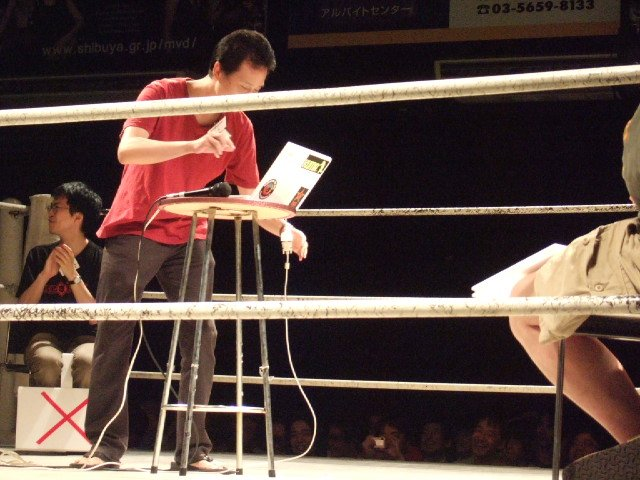
\includegraphics[width=1\hsize]{image200609/20060827-llgong.jpg}
\end{frame}

\subsection{Debian勉強会}

\begin{frame}
 \frametitle{Debian 勉強会}
 \begin{itemize}
  \item Debian Conference 進捗
  \item Lightning Talks:
	\begin{itemize}
	 \item パッケージメンテナンス遍歴から見たDebian史 野首さん
	 \item IPv6 吉田@板橋さん
	 \item 30愁年を迎えて 山下さん
	 \item module-assistant パッケージ作成方法
	 \item board@jpお仕事日記
	\end{itemize} 
 \end{itemize}
\end{frame}

\subsection{i18n conference}

\begin{frame}{i18n conference}
武藤さんが参加したそうです\\
来月報告あるかも?
\end{frame}

\section{あなたが知らないうちに使っているDebian specific}
\begin{frame}{あなたが知らないうちに使っているDebian specific}
 
\end{frame}

\section{翻訳のすすめ}
\begin{frame}{翻訳のすすめ}
 
\end{frame}

\section{dpkg, apt のプロファイリング}
\begin{frame}{dpkg, apt のプロファイリング}
 \begin{itemize}
  \item profiling ってなに?
  \item oprofie のインストールと設定方法
  \item デバッグシンボル
  \item プロファイルの仕方
  \item 結果を見てみる
 \end{itemize}
\end{frame}

\subsection{profilingってなに?}
\begin{frame}{profilingってなに?}
\begin{enumerate}
 \item コンピュータ・ソフトウェア開発において、実行速度のボトルネックを
       調べるなどの目的の為に、プログラムの実行速度をモジュール単位で詳
       細に分析することである。それに用いられるツールをプロファイラーと
       いう。
 \item 犯罪捜査において、犯罪の性質や特徴から、行動科学的に分析し、犯人の特徴を推定すること
\end{enumerate}
Wikipedia より
\end{frame}

\subsection{oprofile のインストールと設定方法}
\begin{frame}{oprofile のインストールと設定方法}
カーネルがサポートしていることを確認。

\texttt{Intrumentation support : Profiling Support :
Oprofile system profiling (experimental)}

\begin{center}
 \texttt{apt-get install oprofile}
\end{center}
\end{frame}


\subsection{デバッグシンボル}
\begin{frame}{デバッグシンボル}

デバッグシンボルがないと、プロファイルが実行ファイル単位にでてくる。
関数単位にするためには、デバッグシンボルつきでコンパイル。

\texttt{debuild -e DEB\_BUILD\_OPTIONS=nostrip}

\end{frame}

\subsection{プロファイルの仕方}
\begin{frame}{プロファイルの仕方}

opcontrol コマンドを活用、スクリプトを事前に作成しておく。

\end{frame}

\subsection{結果を見てみる}
\begin{frame}{結果を見てみる}

関数毎にどれくらい負荷がかかっているか見れます

\texttt{opreport -l }

\end{frame}

\subsection{まとめ}
\begin{frame}{まとめ}
\begin{itemize}
 \item プロファイリングすれば重い処理がわかり、
       最適化の手がかりになる
 \item 実はプロファイルを取得するのはそんなにむずかしくない
 \item みんなで最適化するしか!
\end{itemize}
\end{frame}


\section{LLGONG発表報告}
\begin{frame}{LLGONG発表報告}

\end{frame}

\section{グループワーク}

\begin{frame}
 \frametitle{今後のイベントの検討}
 \begin{itemize}
  \item Debian 勉強会の目的:
  \item イベントにより期待する効果:
  \item 必要な行動:
 \end{itemize}
\end{frame}

\begin{frame}
 \frametitle{今後のイベント}
 \begin{itemize}
  \item OSC-Fall 10月28日? 
  \item OSC 沖縄 12月1日?
  \item KOF 11月18日
  \item Debian 勉強会大阪開催 11月19日
  \item Debian Conference 2007 Edinburgh 2007年6月
  \item Debian 14周年 2007年8月16日
  \item Debian 15周年 2008年8月16日
 \end{itemize}
\end{frame}

\section{wrap-up}
\begin{frame}
 \frametitle{今日のまとめ}
 \begin{itemize}
  \item まとめ
 \end{itemize}
\end{frame}


\end{document}
